\section{Cortex-M}
\subsection{Aligned/Unaligned Data}
Daten auf dem Stack sollten immer Aligned sein, um einen schnellen Zugriff zu gewährleisten. Das bedeutet, dass eine Adresse bei einem 32bit breite Stack durch 4 Teilbar sein muss. Um schnell herauszufinden, kann die letzte Hex Stelle bewertet werden, falls diese $0,4,8,C$ ist, dann wird die Adresse aligned sein. Für Binäre Adressen müssen die letzten Zwei Bits 0 ($(adr \& 0x03) == 0 \xrightarrow{} unaligned$)  sein! Pro Byte-Zugriff wird 1 Zyklus benötigt.
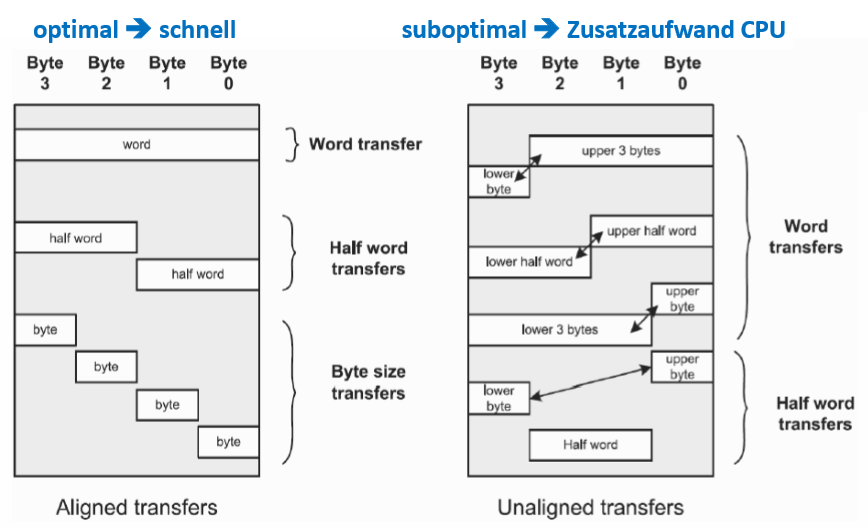
\includegraphics[width=\columnwidth]{Images/aligned}

\subsection{Byteanordnung}
\textbf{ACHTUNG}: Folgende Abbildung ist ein \textbf{1-Byte} organisierter Speicher! Überlicherweise sind Cortex-M Little-Endian Geräte, können aber umkonfiguriert werden.
\begin{center}
	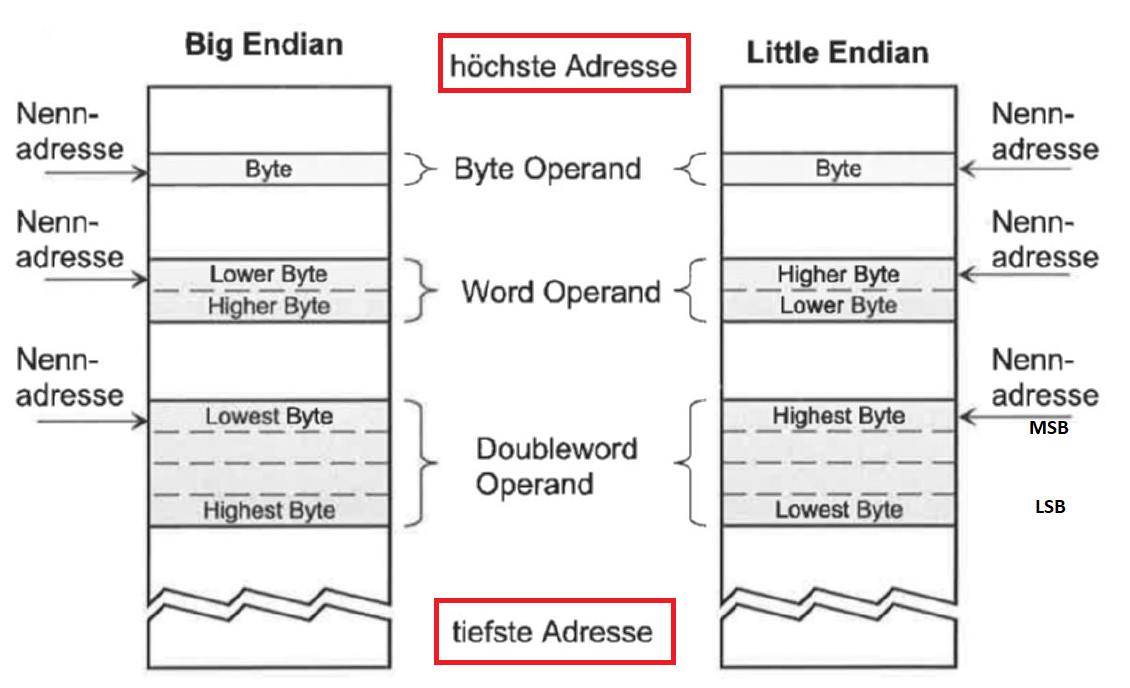
\includegraphics[width=\columnwidth]{Images/byteanordnung}<
\end{center}


\subsection{Bit-Banding}
Bit-Banding ist ein Feature, welches dem Anwender erlaubt auf einzelne Bits direkt via. zB $LDR$ oder $STR$ Befehle zuzugreifen. Dies kann verwendet werden um, zB herauszufinden ob ein GPIO Pin auf High bzw. Low ist, oder ein einzelnes Bit setzen, ohne zu Maskieren. Immer checken, ob Perepherie oder SRAM Zugriff gilt, andere BBAB bzw BBRB Adressen. \textbf{Siehe QuickRef Kapitel Bit-Banding}!
\noindent\textbf{Beispiel 1}: Bit-Nr.7 der Speicherstelle $0x2000'0010$ soll Zugegriffen werden
\begin{align*}
	a &= MA - BBRB \xrightarrow{} 2000'0020_{16} - 2000'0000_{16} = 0010_{16} \\
	b &= a \overbrace{\cdot 32}^{<< 5} \xrightarrow{} 0010_{16} << 5 = 200_{16}\\
	c &= 7 \overbrace{\cdot 4}^{<< 2} \xrightarrow{} 07_{16} << 2_{16} = 1C_{16} \\
	\\
	Address &= 0x2200'0000 + 0x0200 + 0x001C = 0x2200'021C
\end{align*}

\noindent\textbf{Beispiel 2}: Welches Bit wird mit der Addresse $0x2200'8004$ geändert?
\begin{align*}
	Bit &= (Address \overbrace{/4}^{>> 2}) \text{ \& } 7_{16} \\
	    &= 8802'2001_{16} \text{ \& } 7_{16} = 1 \\
	MA &= BBRB + ((Address - BBAB) \overbrace{/ 32}^{>> 5}) \\
	   &= 2000'0000_{16} + ((2200'8004_{16} - 2200'0000_{16}) >> 5)\\
	   &= 2000'0400_{16}
\end{align*}

\subsection{Instructions}
\subsubsection{IT}
$IT$ kann verwendet werden um weniger Code zu schreiben.
\begin{center}
	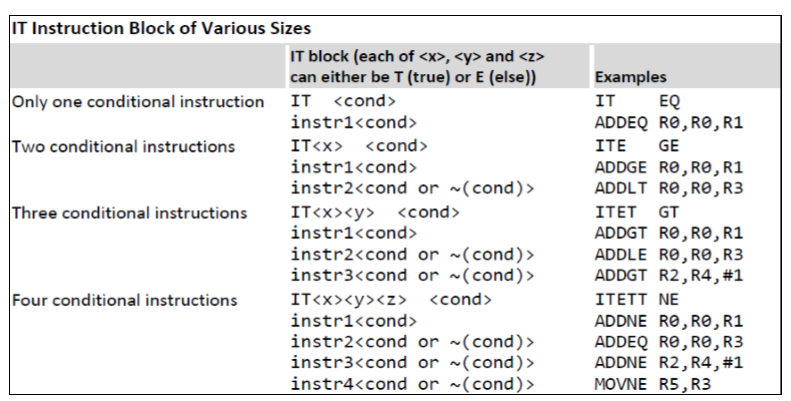
\includegraphics[width=0.9\columnwidth]{Images/IT}
\end{center}
\subsubsection{Conditional}

\begin{center}
	\rotatebox{90}{
		\bgroup
		\def\arraystretch{2.5}
		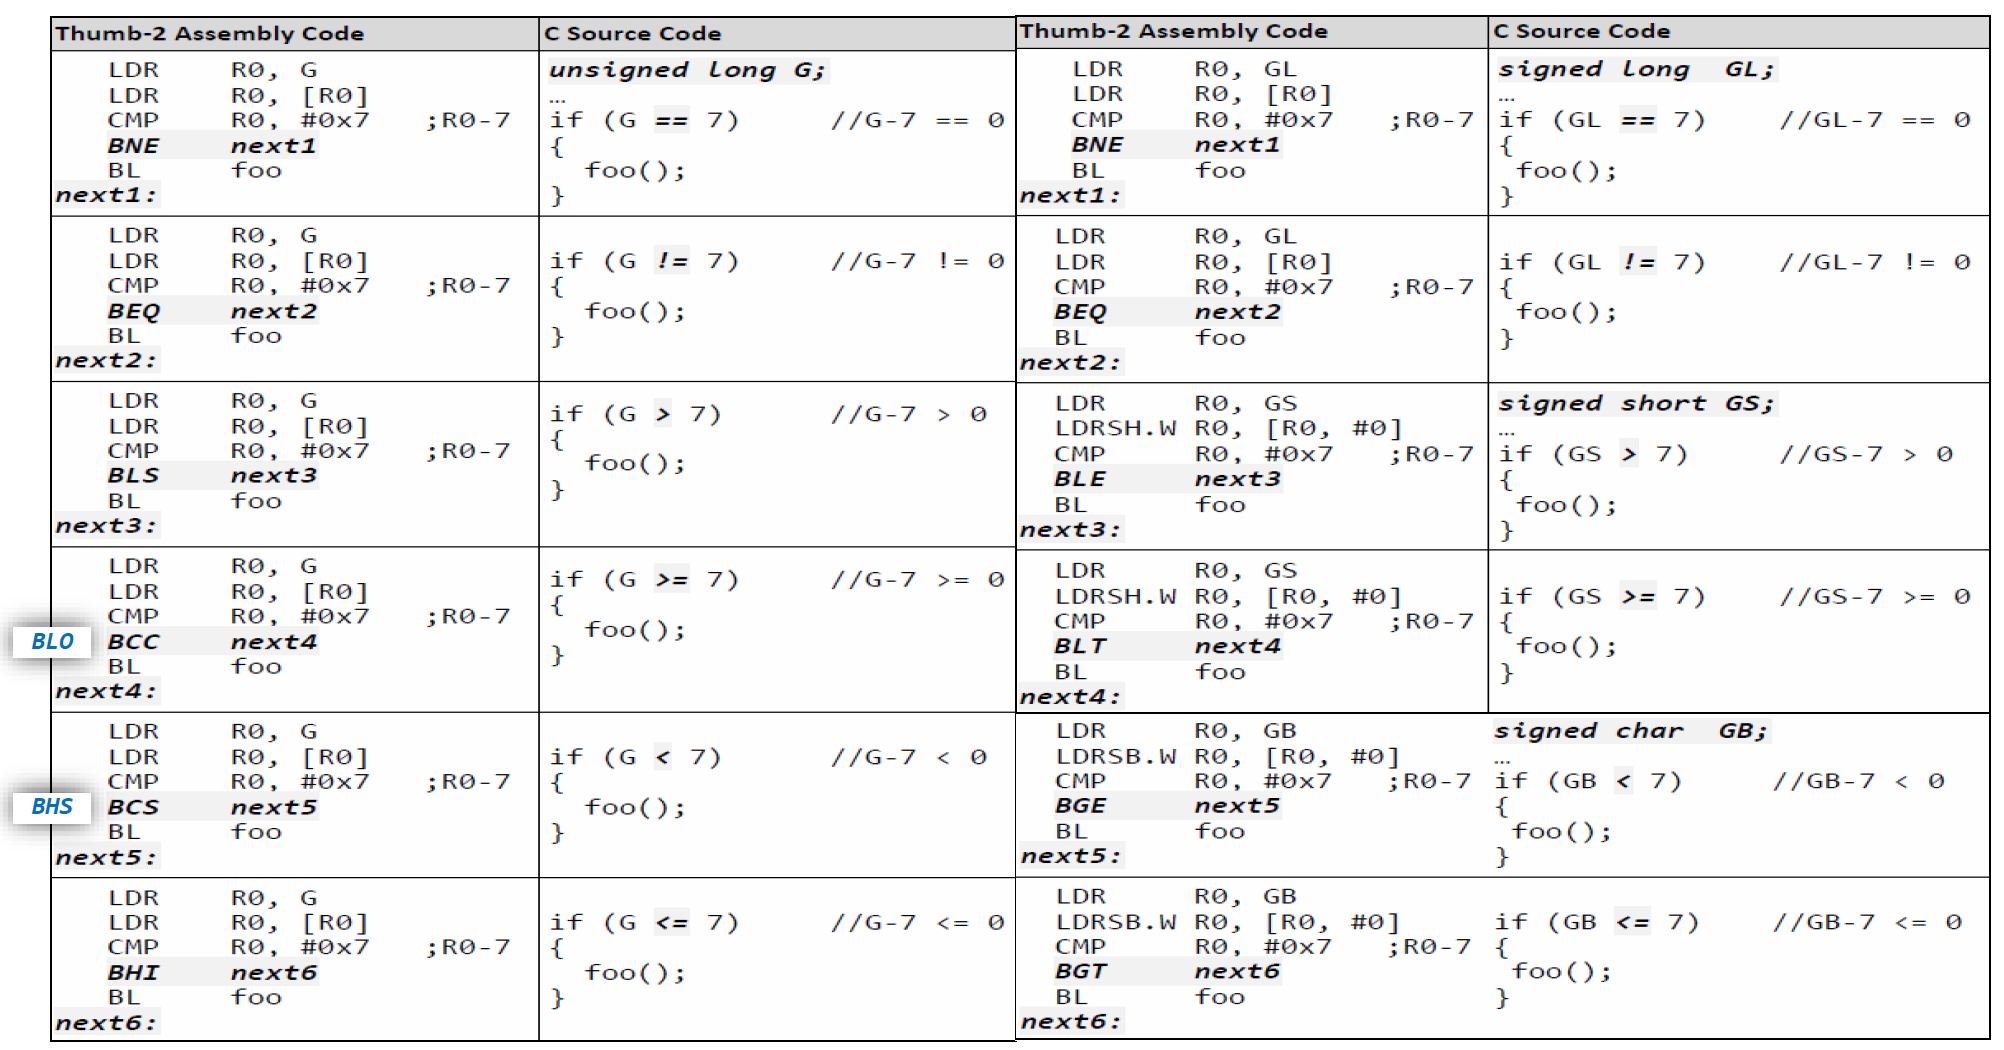
\includegraphics[height=\columnwidth]{Images/conditional}
		\egroup
	}
\end{center}

\subsection{Optimierung}
\begin{itemize}[nosep]
	\item Arrays mit Pointer ersetzen
	\item Loops gegen 0 dekrementieren ($--i$ nicht $i--$)
	\item Assembler Befehle optimieren (zB SIMD)
	\item Loop unrolling
\end{itemize}

\subsection{USART}
\subsubsection{Parallel vs Seriel}
Serielle werden Daten nacheinander geschickt, parallel über mehrere Leitungen gleichzeitig. Die Baudrate sind $\frac{1}{s}$ übertragenen Bits.

\subsubsection{Datenkanäle}
\begin{center}
	\includegraphics[width=\columnwidth]{Images/datenkanäle}
\end{center}

\subsubsection{Datenframe}
Typische \textbf{Baudraten} sind 9600 ($104.2\mu s$), 19200 ($52.08\mu s$), 115200 ($8.68\mu s$). Die \textbf{Daten-Bits} 5..8Bit und \textbf{Parity} ist Even/Odd or None, Anzahl \textbf{Stop-Bit} 1/1.5/2

\noindent Die \textbf{Nutzdatenrate} kann berechnet werden mit für 9600Baud, Odd Parity, 7 Daten-Bit und 2 Stop-Bit. Was 11 Byte pro Frame umfasst (1 Start + 7 Data + 1 Parity + 2 Stop = 11 Bit)
\[
NR = \frac{7Bit \cdot 9600bit/s}{11 Bit}\cdot \frac{1Byte}{8Bit} = 763.63Byte/s
\]

\noindent \textbf{Signalabfolge} für Beispiel von oben. \textbf{Achtung}: Bitreihenfolge ist von links nach rechts! zB Data $W = 0b1010111$
\begin{center}
	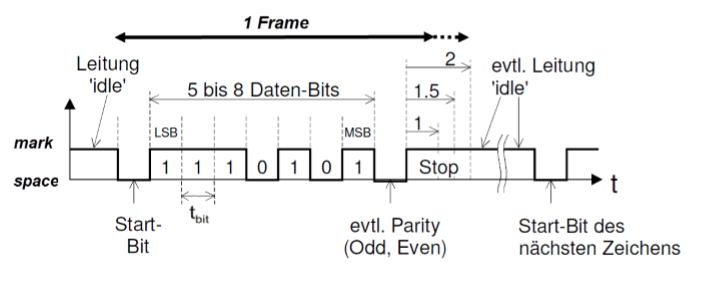
\includegraphics[width=\columnwidth]{Images/datenframe}
\end{center}
Das Parity kann nach folgendem Schema berechnet werden:\\
\begin{center}
	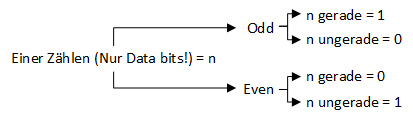
\includegraphics[width=0.8\columnwidth]{Images/parity}
\end{center}

